\chapter{Flujo de uso del panel}
\label{app:flujo-prototipo}

Este anexo amplía la descripción del panel presentada en la sección~\ref{sec:prototipo-inspeccion}. Las pantallas muestran cómo se prepara una ejecución y cómo se consultan sus resultados; no representan un flujo de publicación dentro de un LMS.

El acceso comienza en una página informativa pública\footnote{\url{https://magrimal.github.io/tfm-2026-discussion-moderation/}} separada del panel (figura~\ref{fig:landing-page}). Esta página resume el propósito del proyecto y explica las tres operaciones principales: clasificar el hilo, decidir si intervenir y generar una propuesta cuando corresponde. También enlaza los dos despliegues experimentales del mismo sistema: Idril, el servidor de la Facultad de Informática que ejecuta modelos locales mediante Ollama, y AWS EC2, la instancia que accede a modelos externos y se publica bajo el dominio \texttt{facilitation.mgmdy.xyz}. La página identifica este segundo despliegue como \emph{MGMDY} por el dominio y lo presenta junto al entorno de Idril. Desde las tarjetas se abre el panel desplegado en cada servidor. El acceso está protegido mediante autenticación HTTP básica.

\begin{figure}[htbp]
\centering

\includegraphics[width=0.85\textwidth]{figures/landing-page-tfm}
\caption{Página de entrada al proyecto, con los dos entornos experimentales y un resumen del funcionamiento.}
\label{fig:landing-page}
\end{figure}

\FloatBarrier
Dentro del panel, la navegación se concentra en dos opciones: \emph{New run}, para crear una ejecución, y \emph{Runs}, para consultar las anteriores. \emph{New run} presenta cuatro bloques desplegables (figura~\ref{fig:new-run-threads}). Primero se elige entre \emph{Sample data}, los hilos incluidos con el proyecto, y \emph{Live course}, que carga una instantánea de un curso. Después se revisan los hilos disponibles y se marcan los que formarán parte de la ejecución. Cada hilo puede abrirse antes de seleccionarlo.

\begin{figure}[htbp]
\centering
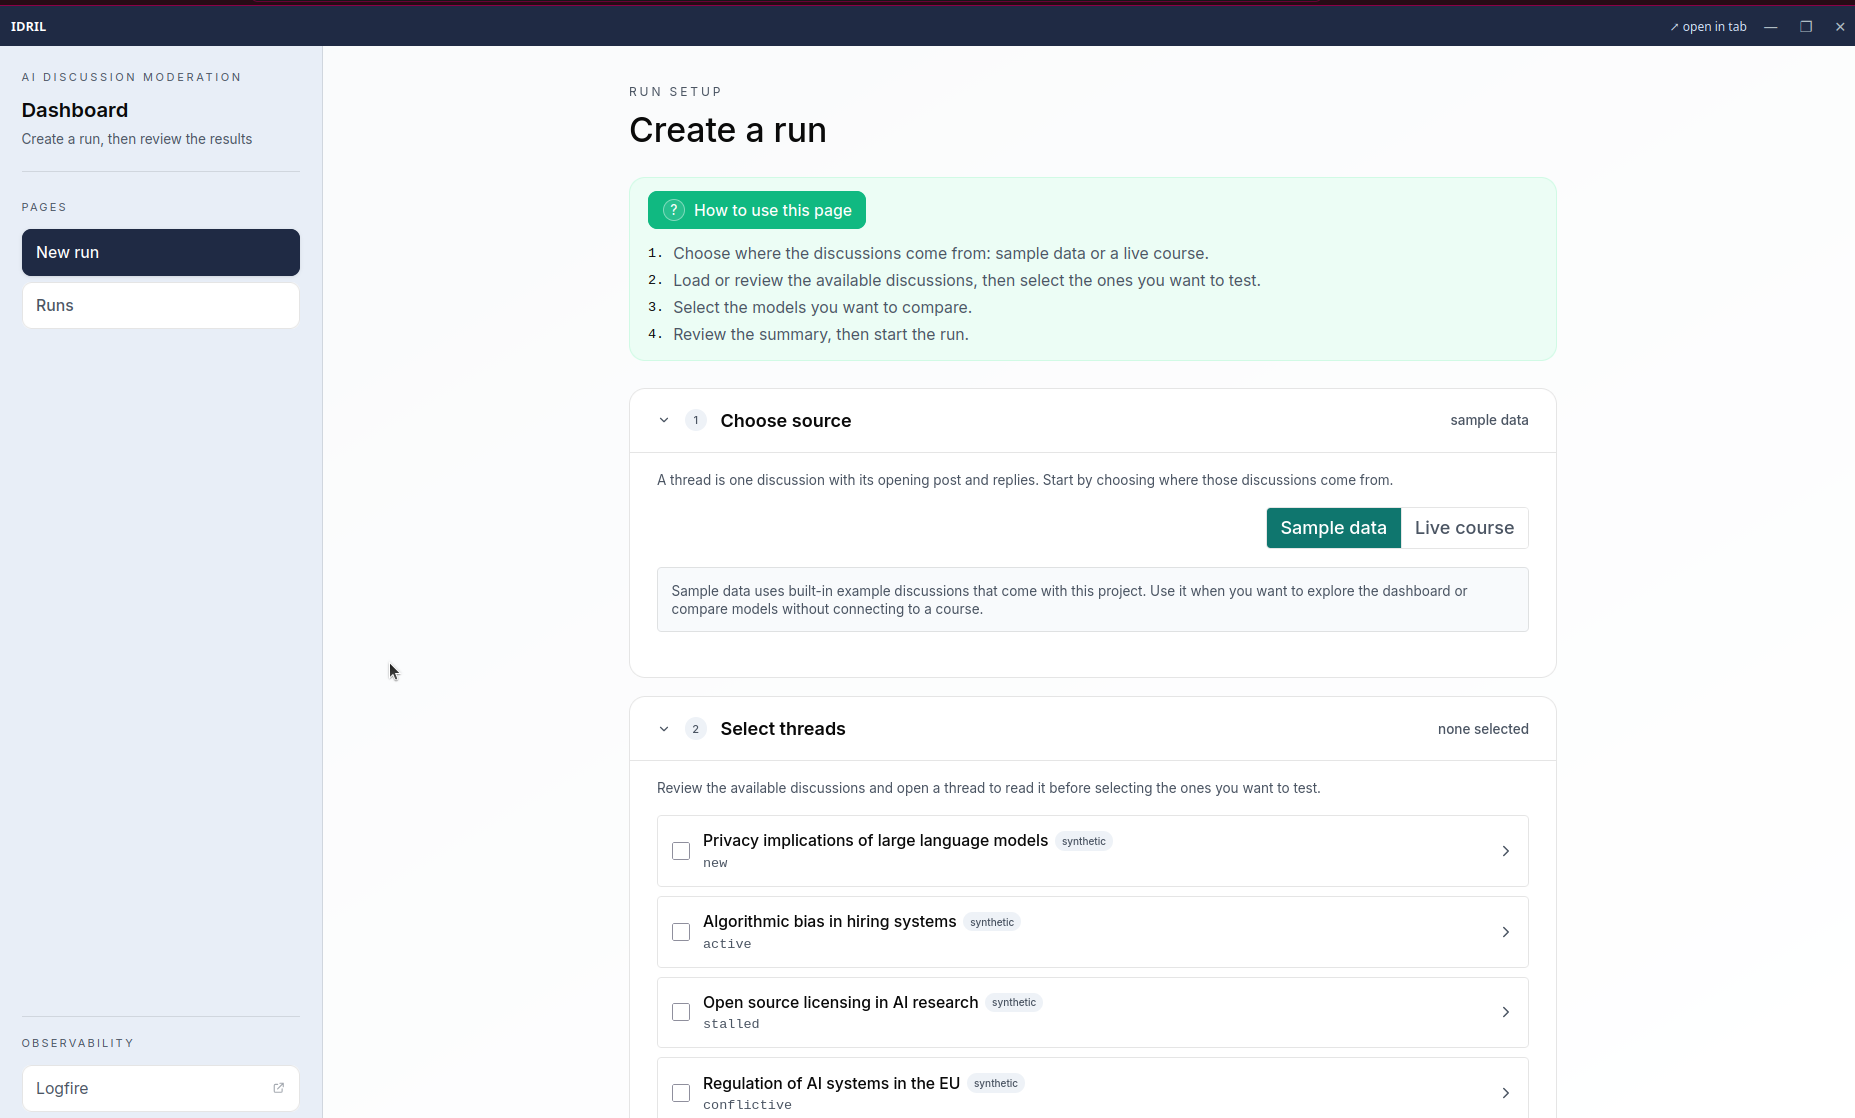
\includegraphics[width=0.95\textwidth]{figures/dashboard-new-run-threads-latest}
\caption{Primeros pasos de una ejecución: elección de la fuente y selección de hilos.}
\label{fig:new-run-threads}
\end{figure}

\FloatBarrier
El tercer bloque selecciona los modelos que se compararán y el cuarto resume el número de hilos, modelos y comparaciones antes de iniciar la ejecución (figura~\ref{fig:new-run-models}). El tamaño del experimento es el producto de los hilos y modelos seleccionados. Al iniciarlo, sus resultados se guardan para inspección.

\begin{figure}[htbp]
\centering
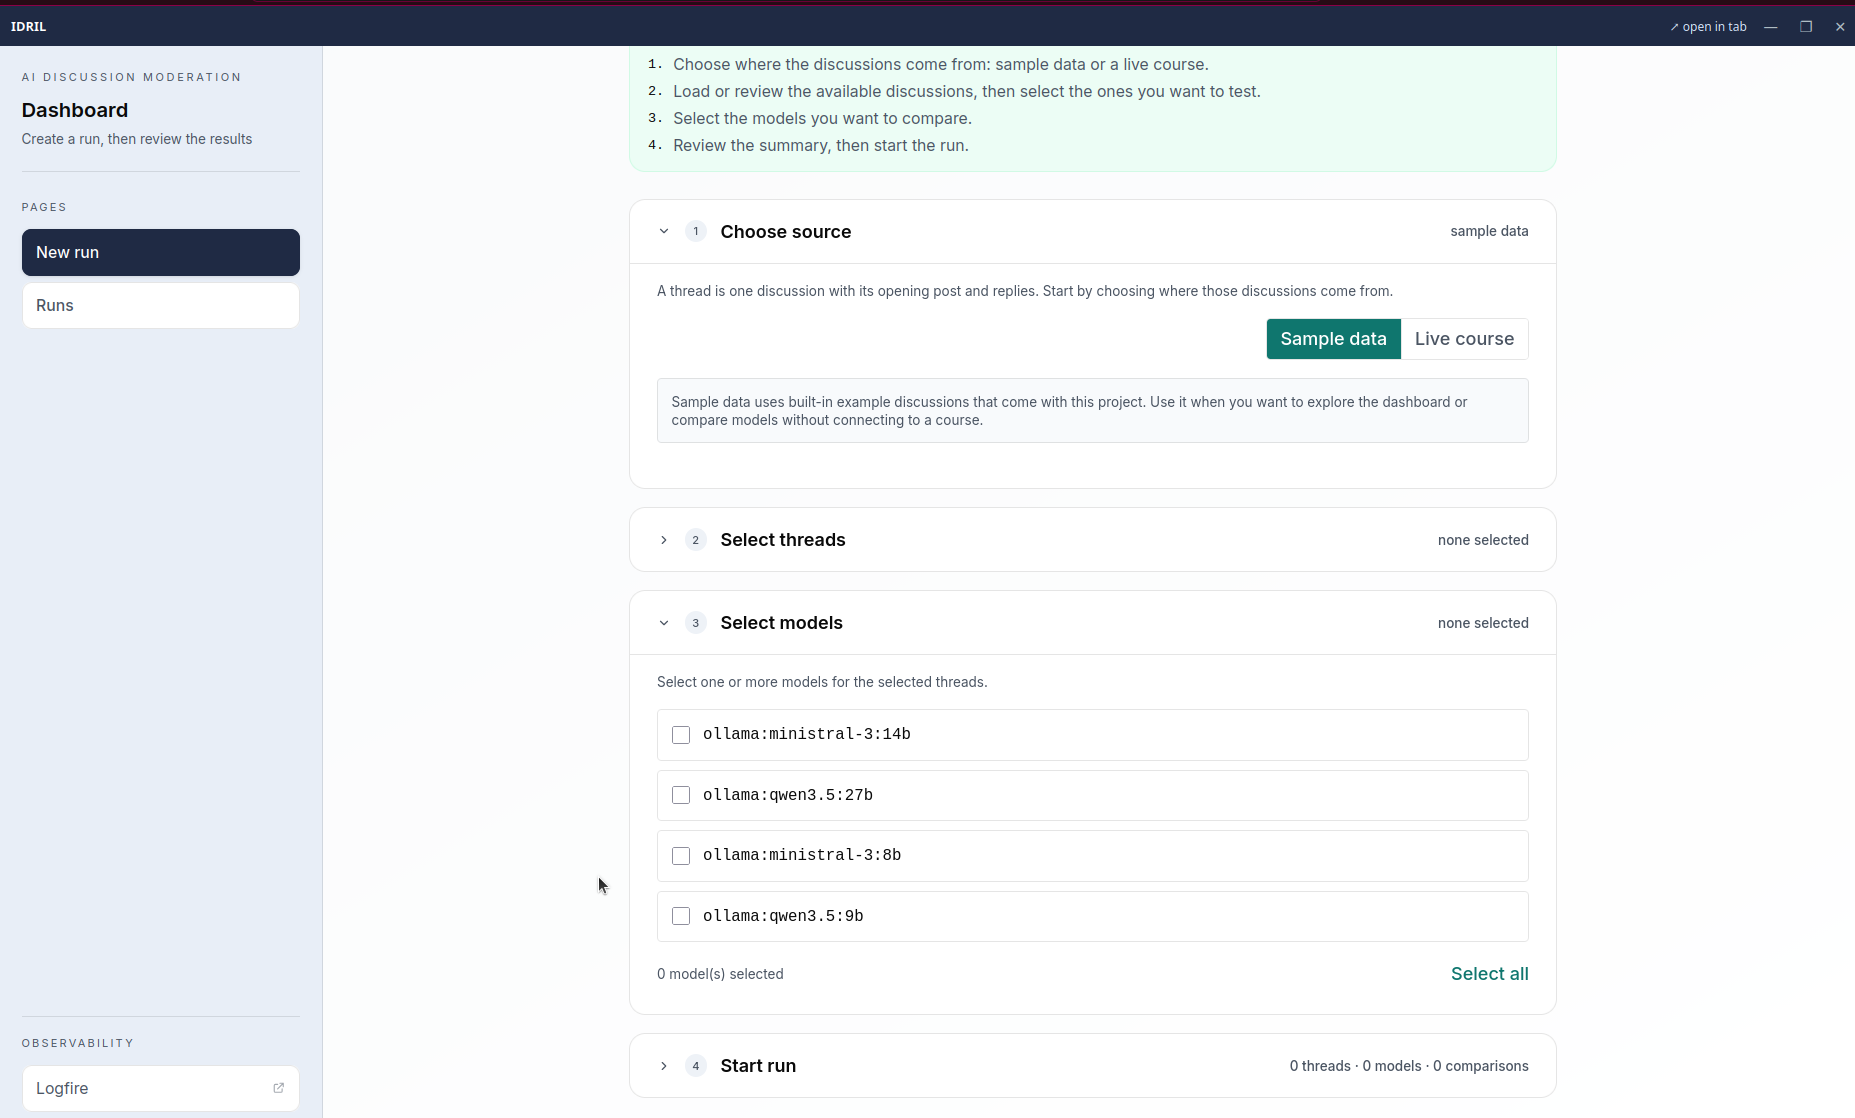
\includegraphics[width=0.95\textwidth]{figures/dashboard-new-run-models-latest}
\caption{Selección de modelos y resumen del número de comparaciones antes de iniciar la ejecución.}
\label{fig:new-run-models}
\end{figure}

\FloatBarrier
La opción \emph{Runs} abre el historial (figura~\ref{fig:run-history}). Cada fila muestra el nombre y la fecha de la ejecución, cuántas comparaciones terminaron y su estado. Una ejecución puede aparecer terminada, cancelada o interrumpida por el reinicio del servicio. Al abrirla, el panel muestra primero un resumen con el número de modelos, evaluaciones ejecutadas y errores. Debajo aparece la comparación por modelo, con ejecuciones completadas, velocidad media, errores y un enlace al detalle (figura~\ref{fig:run-overview}). También se puede preparar una nueva ejecución con la misma configuración mediante \emph{Retry run}.

\begin{figure}[htbp]
\centering
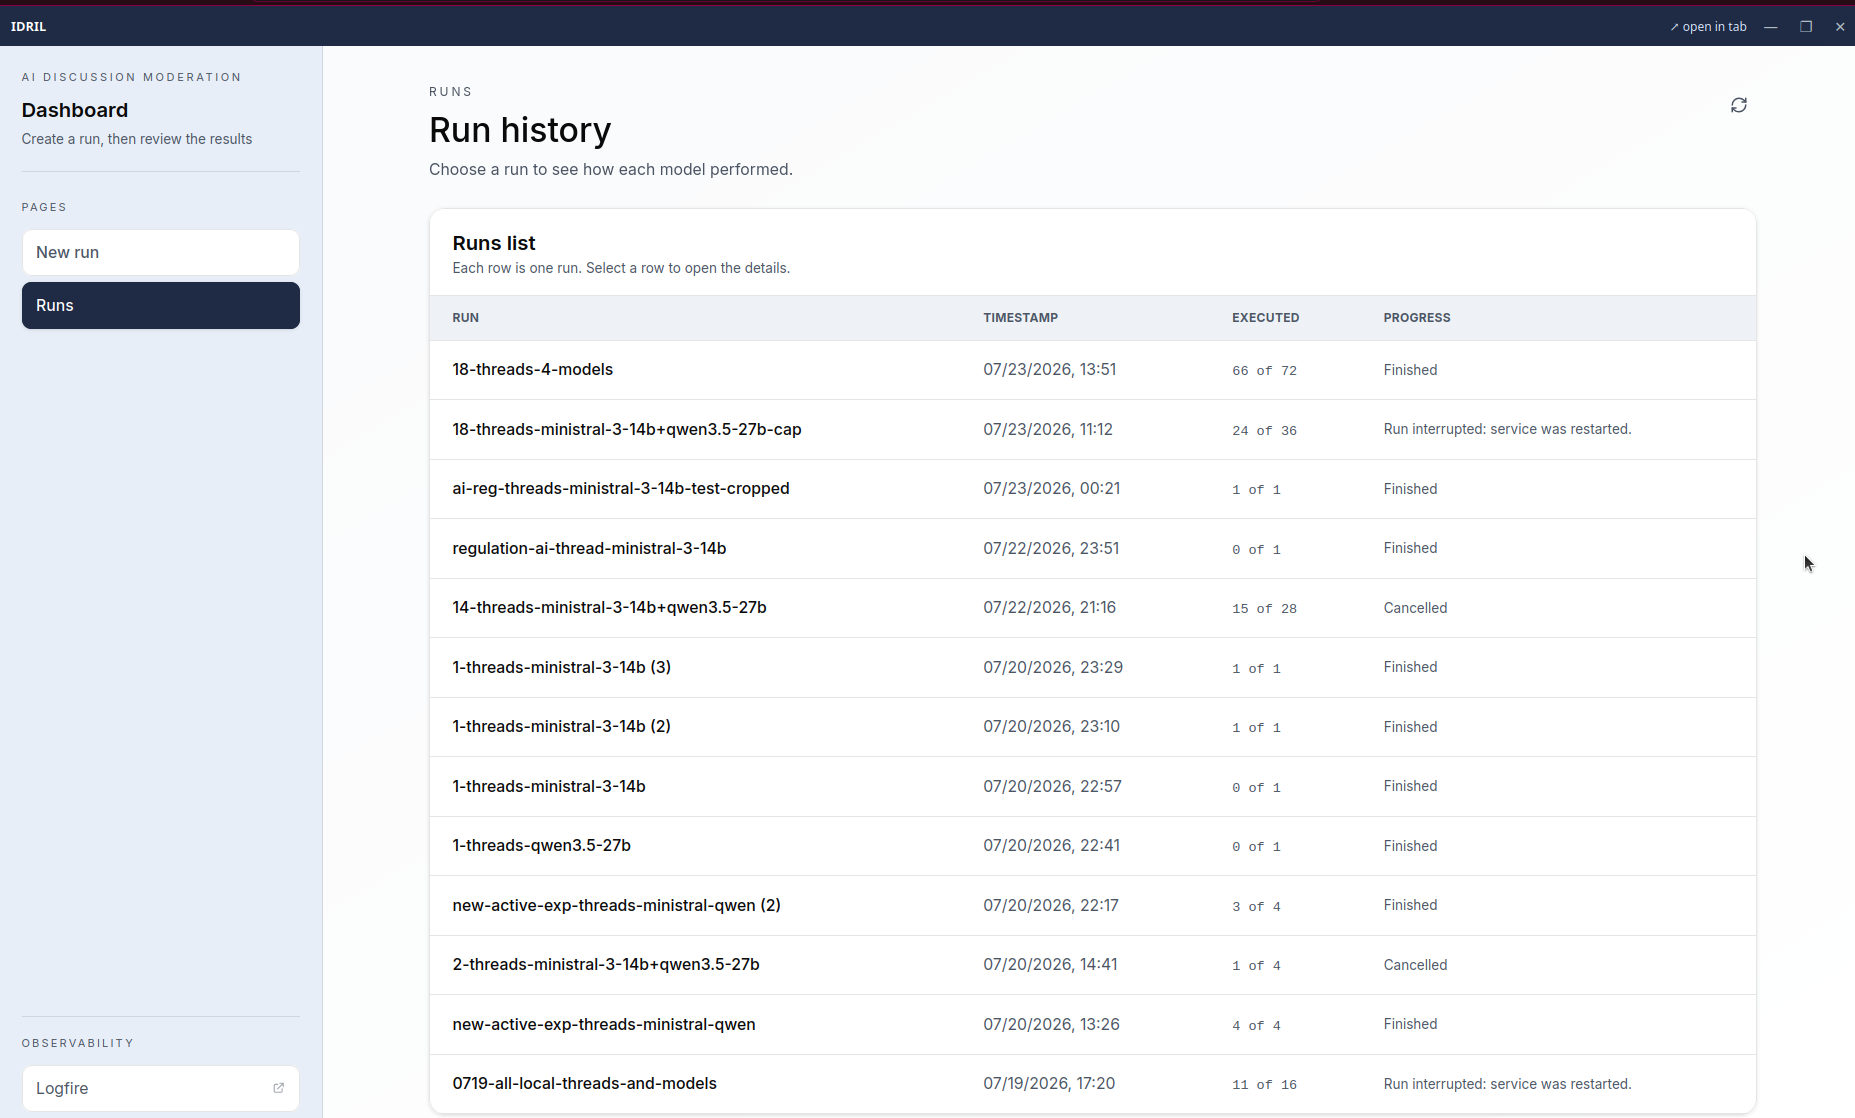
\includegraphics[width=0.95\textwidth]{figures/dashboard-run-history-latest}
\caption{Historial de ejecuciones con progreso y estado final.}
\label{fig:run-history}
\end{figure}

\begin{figure}[htbp]
\centering
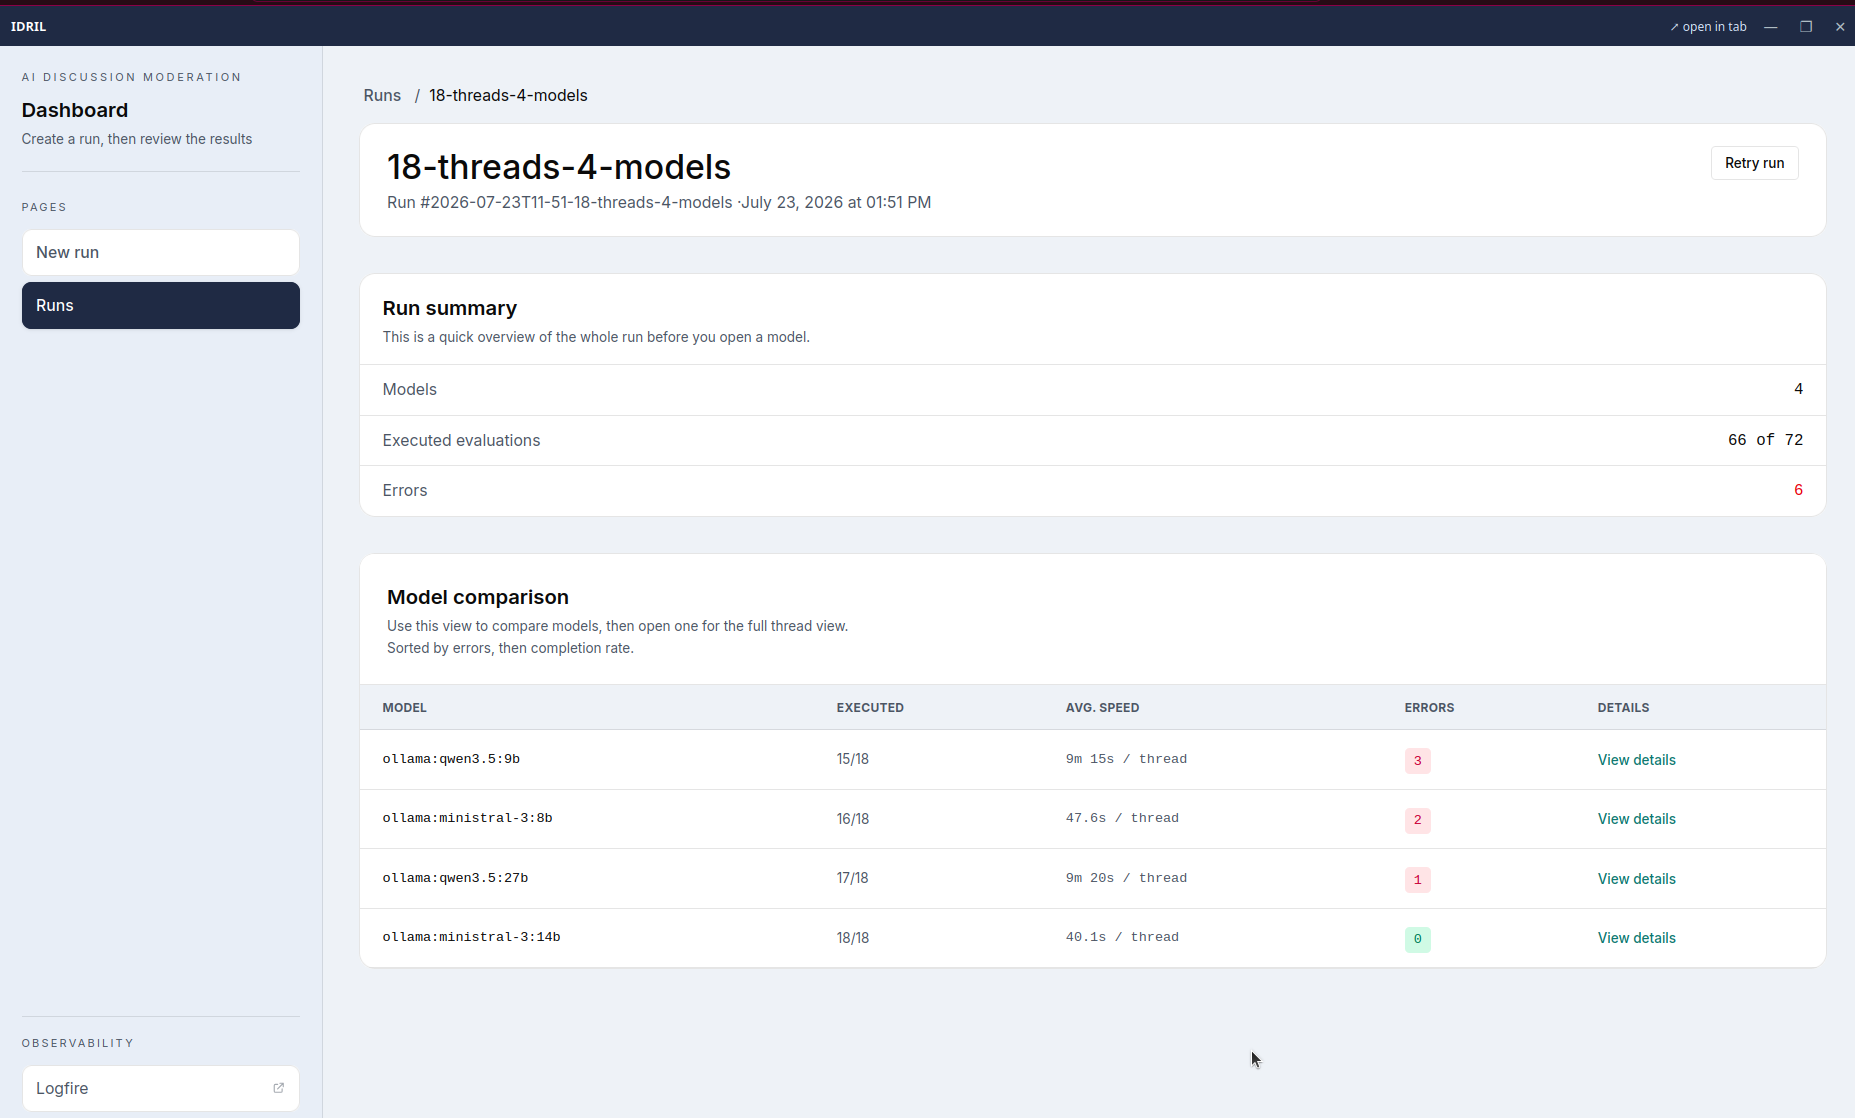
\includegraphics[width=0.95\textwidth]{figures/dashboard-run-overview-latest}
\caption{Resumen de una ejecución y comparación de completitud, velocidad y errores por modelo.}
\label{fig:run-overview}
\end{figure}

\FloatBarrier
Al abrir un modelo, el panel indica la fuente de los hilos, resume su completitud, número de acciones sugeridas, errores y velocidad media, y presenta la lista de hilos revisados (figura~\ref{fig:model-detail}). Cada fila anticipa la predicción y si el modelo propone intervenir. Estas etiquetas son resultados del modelo; cuando existe una clasificación local de referencia, la interfaz la presenta solo como orientación y no como verdad de referencia.

\begin{figure}[htbp]
\centering
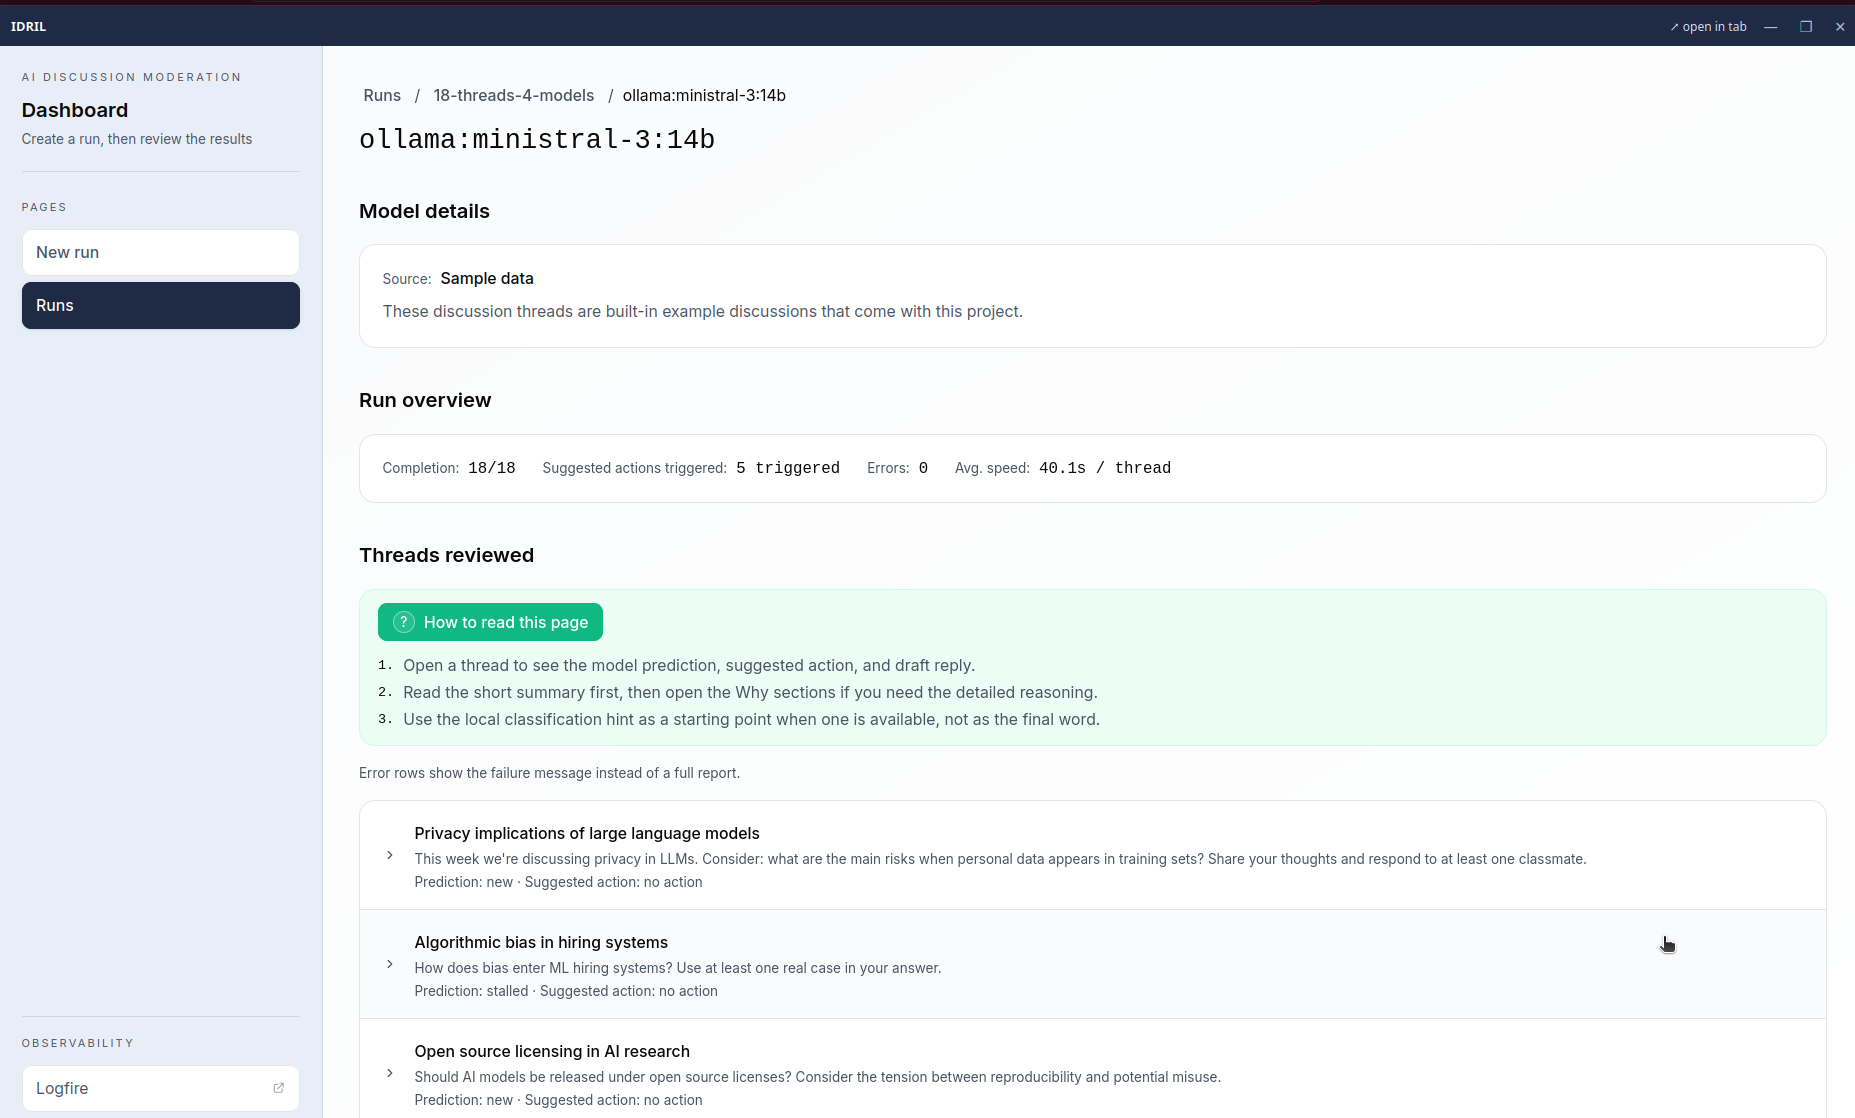
\includegraphics[width=0.95\textwidth]{figures/dashboard-model-detail-latest}
\caption{Detalle de un modelo dentro de una ejecución y lista de hilos revisados.}
\label{fig:model-detail}
\end{figure}

La vista final de cada hilo, con la discusión, la predicción, la acción sugerida y la respuesta candidata, se muestra en la figura~\ref{fig:thread-analysis}.
